\documentclass[letterpaper]{article}
\title{CSE446 Machine Learning, Winter 2016: Homework 1}
\date{Due: Monday, January $25^{th}$, beginning of class}
\usepackage{hyperref}

\usepackage[margin=1in]{geometry}

\usepackage{amsmath,amsfonts}
\usepackage{capt-of}
\usepackage{url}
\usepackage{graphicx}
\usepackage{color}
\usepackage{bbm}
\usepackage{enumerate}
\newcommand{\carlos}[1]{\textcolor{red}{Carlos: #1}}
\newcommand{\field}[1]{\mathbb{#1}} 
\newcommand{\hide}[1]{#1}
\newcommand{\pd}[2]{\frac{\partial #1}{\partial #2}}
\providecommand{\m}[1]{\mathbf{#1}}
\providecommand{\norm}[1]{\left\|#1\right\|}
\providecommand{\sign}[1]{\text{sign}\left(#1\right)}
\DeclareMathOperator*{\argmin}{arg\,min}
\providecommand{\what}{\m{\hat{w}}}
\providecommand{\dw}{\Delta w}
\providecommand{\dmw}{\Delta \m{w}}
\providecommand{\hy}{\hat{y}}
\usepackage[ruled]{algorithm2e}

\hypersetup{
    colorlinks=true,
    linkcolor=blue,
    filecolor=blue,      
    urlcolor=blue,
}
 
\begin{document}
\author{\href{github.com/gshguru}{Gurupad S. Hegde} }
\maketitle

\noindent Start Early! Also, typed solutions (specifically those in LaTeX) are preferred to hand-written solutions. Any illegible solutions will be counted wrong at the sole discretion of the grader. Please feel free to use the homework document as a template, putting your solutions inline. We will only accept answers in \textbf{.pdf} format. 

\section{Probability Review [30 points]}
\begin{enumerate}
\item You are just told by your doctor that you tested positive for a serious disease. The test has 99\% accuracy, which means that the probability of testing positive given that you have the disease is 0.99, and also that the probability of testing negative given that you do not have the disease is 0.99. The good news is that this is a rare disease, striking only 1 in 10,000 people.

\begin{enumerate}[a]
\item (5 points) Why is it good news that the disease is rare?\\
Its given that Probability of occurrence is rare i.e. of probability 0.0001. This reduces the risk of being impacted by a disease because of very low prior.  When we compare this with test accuracy, this is very very low. So, there is a greater chance that you might have not infected by disease. 
\item (10 points) What are the chances that you actually have the disease? Show your work.
\begin{flalign*}
&P(T^+|D^+) = 0.99 &\\ 
&P(T^-|D^-) = 0.99 &\\
&P(D^+) = 0.0001 &\\ 
&P(D^-) = 0.9999 &\\
&P(T^+) = P(T^+|D^+)*P(D^+) + P(T^+|D^-)*P(D^-) = 0.99*0.0001  + 0.01*0.9999 = 0.010098 &\\
&P(D^+|T^+) = \frac{ P(T^+|D^+) * P(D^+) } {P(T^+)} \frac{0.99  * 0.0001}{0.010098 } = \textbf{0.0098}
\end{flalign*}

\end{enumerate}

\item A group of students were classified based on whether they are senior or junior and whether they are taking CSE446 or not. The folowing data was obtained.
\begin{center}
  	\begin{tabular}{|c|c|c|}
  	\hline
  	 & Junior & Senior \\
  	\hline
  	taking CSE446 & 23 & 34 \\
  	\hline
    no CSE446 & 41 & 53 \\
  	\hline
  	\end{tabular}
\end{center}
Suppose a student was randomly chosen from the group. Let $J$ be the event that the student is junior, $S$ be the event that the student is senior, $C$ be the event that the student is taking CSE446, and $\bar{C}$ be the event that the student is not taking CSE446. Calculate the following probabilities. Show your work.
\begin{enumerate}[a]
\item (5 points) $P(C, S)$
\item (5 points) $P(C | S)$
\item (5 points) $P(\bar{C} | J)$
\begin{flalign*}
\textrm{Prob of taking CSE446 and they are also seniors} 
       &= P(C, S) = \frac{34}{23+34+41+53} = \textbf{0.225} &\\
\textrm{Prob of taking CSE446 among seniors}  
       &= P(C|S) = \frac{34}{53 + 34} = \textbf{0.391} &\\
\textrm{Prob of \textbf{not} taking CSE446 among juniors} 
       &= P(\bar{C}, J) = \frac{23}{23+41} = \textbf{0.359} &\\
\end{flalign*}
\end{enumerate}
\end{enumerate}

\section{Decision Trees [30 points]}
For the first two problems, it would be helpful for you to draw the decision boundary of your learned tree in the figure.
\begin{enumerate}
  \item
  \emph{(14 points)} Consider the problem of predicting if a person has a college degree based on
  	age and salary.  The table and graph below contain training data for 10 individuals.
  	
  \begin{center}
  	\begin{tabular}{|c|c|c|}
  	\hline
  	Age & Salary (\$) & College Degree \\
  	\hline
  	24 & 40,000 & Yes \\
  	53 & 52,000 & No \\
  	23 & 25,000 & No \\
  	25 & 77,000 & Yes \\
  	32 & 48,000 & Yes \\
  	52 & 110,000 & Yes \\
  	22 & 38,000 & Yes \\
  	43 & 44,000 & No \\
  	52 & 27,000 & No \\
  	48 & 65,000 & Yes \\
  	\hline
  	\end{tabular}
   \end{center}
   \begin{center}
   	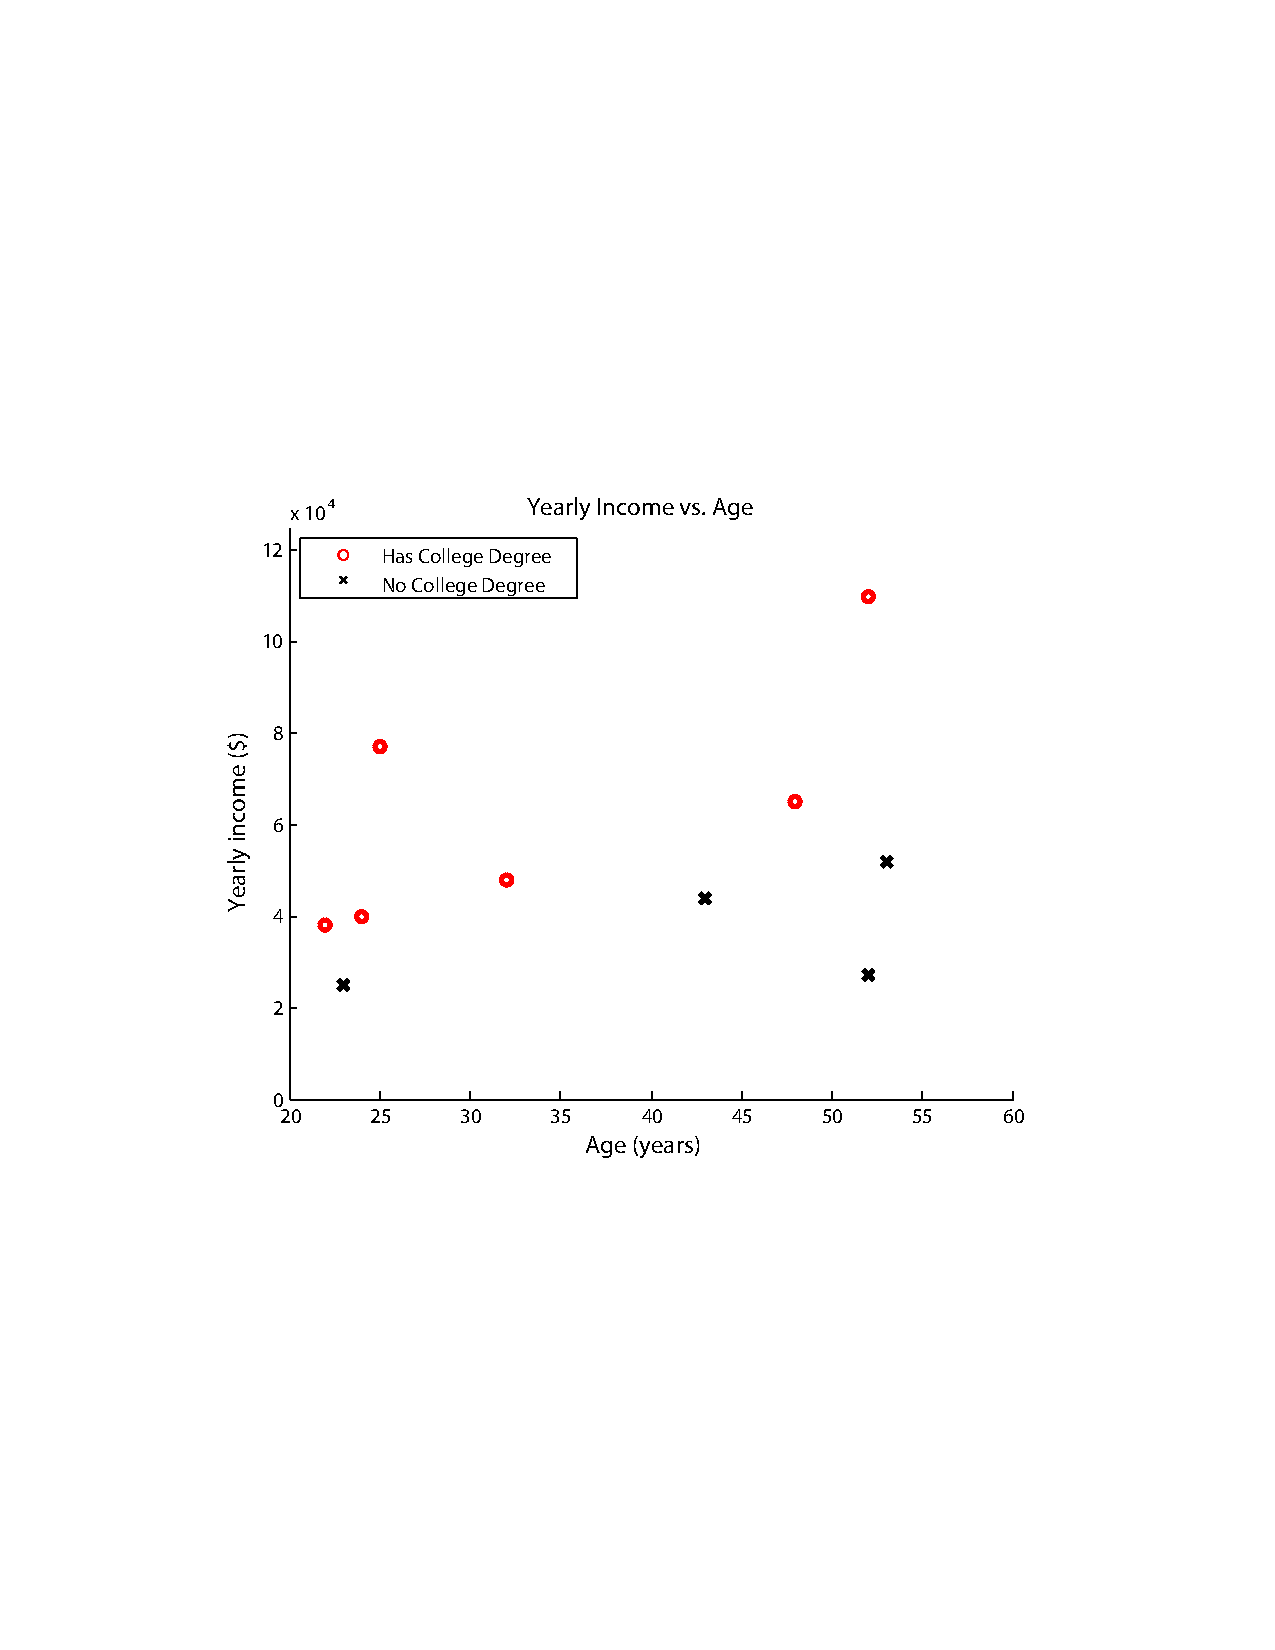
\includegraphics[width=3.5in]{img/hw1-decision-tree.pdf}
   \end{center}
   Build a decision tree for classifying whether a person has a college degree by greedily choosing threshold splits that maximize information gain. What is the depth of your tree and the information gain at each split?
   \\
  \begin{center}
  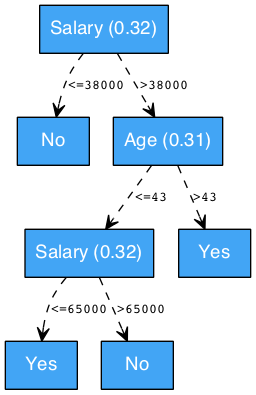
\includegraphics[width=3.5in]{img/dt.png}
  \end{center}
  \item{(12 points)}
  	A multivariate decision tree is a generalization of univariate decision trees, where more than one attribute
  	can be used in the decision rule for each split.  That is, splits need not be orthogonal to a feature's axis.
  	
  	For the same data, learn a multivariate decision tree where each decision rule is a linear classifier that
  	makes decisions based on the sign of $\alpha x_{age} + \beta x_{income} - 1$.
  	
  	Draw your tree, including the $\alpha, \beta$ and the information gain for each split. Include your code with the submission.
  \begin{center}
  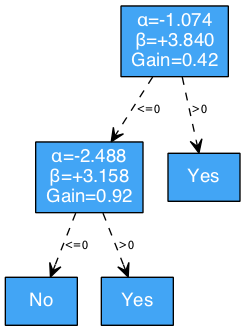
\includegraphics[width=3.5in]{img/mdt.png}
  \end{center}
  \item{(4 points)}
  	Multivariate decision trees have practical advantages and disadvantages.  List an advantage and a disadvantage
  	multivariate decision trees have compared to univariate decision trees.\\
\textbf{Advantage} Splitting can be non-orthogonal to the feature axes. Hence, number of decision rules will be less in such cases compared to univariate decision trees\\
\textbf{Disadvantage} Computationally expensive (like Gradient Decent methods) and models cannot be interpreted as easily as univariate decision tree models
\end{enumerate}

\section{MLE [20 points]}
This question uses a discrete probability distribution known as the Poisson
distribution. A discrete random variable $X$ follows a Poisson distribution
with parameter $\lambda$ if 

\[
\Pr(X=k)=\frac{\lambda^k}{k!}e^{-\lambda}\qquad
k \in \{0,1,2,\dots\}
\]

\noindent
You are a warrior in Peter Jackson's The Hobbit: Battle of the Five Armies. 
Because Peter decided to make his battle scenes as legendary as possible, 
he's decided that the number of orcs that will die with one swing of your sword is Poisson distributed (i.i.d) with parameter
$\lambda$. You swing your sword eight times in the scene. Later, you go see the movie in theaters
and record the number of orcs slain during each swing of your sword:

\begin{center}
\begin{tabular}{l*{8}{c}r}
Sword Swing         & 1 & 2 & 3 & 4 & 5 & 6 & 7 & 8 \\
\hline
Orcs Slain      & 6 & 4 & 2 & 7 & 5 & 1 & 2 & 5\\
\end{tabular}
\end{center}

\noindent
Let $G=(G_1,\dots,G_n)$ be a random vector where $G_i$ is the number
of orcs slain on swing $i$:


\begin{enumerate}
\item \emph{(6 points)} 
Give the log-likelihood function of $G$ given $\lambda$.

\begin{flalign*}
\mathlarger{Pr(G|\lambda)} & 
                 \mathlarger{=\prod_{i=1}^{N} \frac{\lambda^{k_i}}{k_i!}e^{-\lambda}}&\\
\mathlarger{\ln (Pr(G|\lambda))} & 
                 \mathlarger{ = \ln(\prod_{i=1}^{N} \frac{\lambda^{k_i}}{k_i!}e^{-\lambda})}&
\textrm{(Applying} \ln () \textrm{on both the sides)}\quad \\
\mathlarger{\mathcal{L}(\lambda|k)} &
 				\mathlarger{ = \sum_{i=1}^{N}{[\ln{\lambda^{k_i}}   - \lambda\ln e - \ln k_i !]  }}
\mathlarger{ = \sum_{i=1}^{N}\ln{\lambda^{k_i}}  - N\lambda - \sum_{i=1}^{N}\ln k_i !}&\\
&  \mathlarger {=\Big(\sum_{i=1}^{N}k_i\Big) \ln \lambda - N\lambda - \sum_{i=1}^{N}\ln k_i ! }&\\
&\textrm{(Dropping constant term which is not dependent on } \lambda )& \\
\implies
\mathlarger {\mathcal{L}(\lambda|k) } & 
			\mathlarger {=\Big(\sum_{i=1}^{N}k_i\Big) \ln \lambda - N\lambda }&
\end{flalign*}


\item \emph{(8 points)}
Compute the MLE for $\lambda$ in the general case.
\begin{flalign*}
\mathlarger{\frac{d}{d\lambda}  (\ln Pr(G|\lambda)) }&
	\mathlarger{ = \frac{d}{d\lambda} \bigg(  \Big(\sum_{i=1}^{N}k_i\Big) \ln \lambda - N\lambda \bigg)  }&\\
\mathlarger{0} & 
	\mathlarger{ = \frac{\sum_{i=1}^{N}k_i}{\lambda} - N} &
\textrm{(Setting derivative to zero)}\quad \\ 
\implies
\mathlarger{\hat{\lambda}}  &
	 \mathlarger{ = \frac{\sum_{i=1}^{N}k_i}{N}}
\end{flalign*}

\item \emph{(6 point)} 
Compute the MLE for $\lambda$ using the observed $G$.
\begin{flalign*}
&\mathlarger{\hat{\lambda}  = \frac{\sum_{i=1}^{N}k_i}{N} =  \frac{(6+4+2+7+5+1+2+5)}{8} = \textbf{4.0}}&
\end{flalign*}

\end{enumerate}

\section{Programming [100 points]}
Go to https://github.com/pjreddie/C4.5-Homework. \\
\textbf{Solution:} https://github.com/gurupadh/C4.5-Homework

\end{document}
